\section{研究内容介绍}
\label{sec-1}
\begin{frame}[label=sec-1-1]{背景}
\transdissolve<2-4>
\begin{itemize}
\item “大数据”时代来临,我们获得的数据越来越多,研究工作也受到了新的挑战
\item 为了便于计算机处理这些数据,需要从非结构化和半结构化数据中提取出我们关心的
  内容,存储成结构化的数据
\item 大部分网页是通过查询后台数据库,然后选择合适模板进行渲染方式生成的。即:
\end{itemize}
\begin{tikzpicture}[scale=.8, transform shape, node distance=2mm]
  \pause
    \node (template) {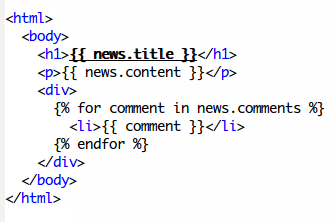
\includegraphics[width=0.5\textwidth]{django}};
  \pause
  \node (arrow) [fill=cyan!50, right=of template, draw, single arrow, minimum height=1cm, minimum width=5mm] {};
  \pause
  \node (webpage)[right=of arrow] {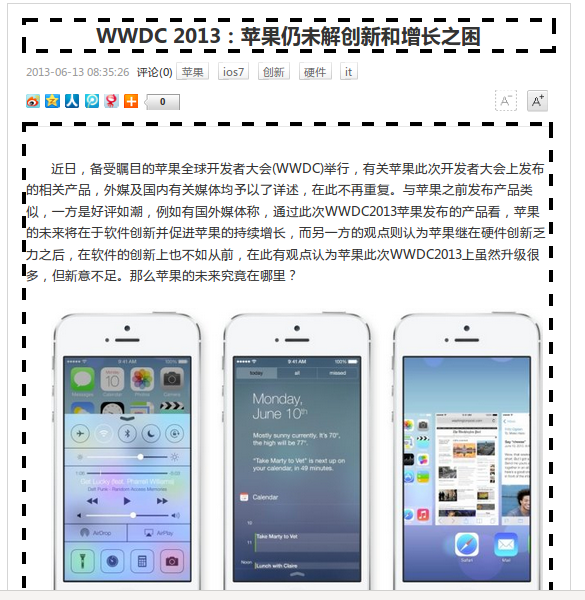
\includegraphics[width=0.5\textwidth]{demoresult}};
\end{tikzpicture}
\end{frame}

\begin{frame}[label=sec-1-2]{工作内容}
  \transblindshorizontal<2-4>
\begin{enumerate}
\item 已经获得大量新闻、博客等网页数据,这些网页可能由不同的模板生成
\item 我们将网页按不同的模板分开,然后从每个集合中提取出所有可能的模板
\item 根据提取出的模板,抽取新的网页中的有用的信息,存储成XML格式。
  \begin{tikzpicture}[scale=.8, transform shape, node distance=2mm]
  \pause
    \node (template) {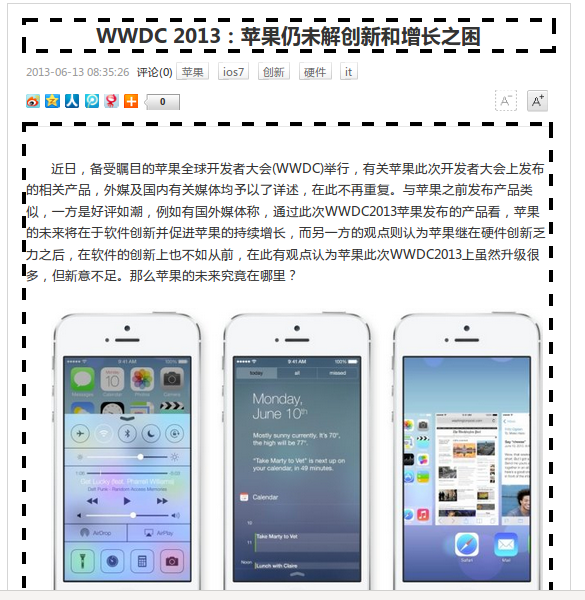
\includegraphics[width=0.5\textwidth]{demoresult}};
  \pause
  \node (arrow) [fill=orange!50, right=of template, draw, single arrow, minimum height=1cm, minimum width=5mm] {};
  \pause
  \node (webpage)[right=of arrow] {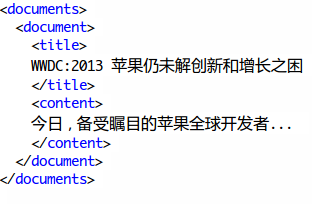
\includegraphics[width=0.5\textwidth]{demoxmloutput}};
\end{tikzpicture}
\end{enumerate}
\end{frame}

%%% Local Variables: 
%%% mode: latex
%%% TeX-master: "../final_report_beamer"
%%% End: 
